\chapter{Measurement Methodology}

This chapter is dedicated to answering the questions of what was measured and how results were obtained. Firstly, the measurement setup is discussed. Secondly,  the GNU Radio flowgraphs are explained. Subsequently, with reference to the flowgraphs measurement metrics are formally defined in view of the necessity to verify the recorded data.  Lastly, an overview of the semi-automatic measurement script system designed to automate, therefore accelerate the process of file system management, data processing and result plotting is given.

\section{Measurement Setup}

The setup consists of two USRP2s from Ettus Research and two USRP 2920s from National Instruments. The former pair is programmed as receiver and sniffer, whereas the latter as senders as depicted in \ref{fig:measurement-setup}. Each USRP was connected to a gigabit switch through a LAN cabel. The scripts running on the devices were launched from a local computer with the IP 134.130.223.151, which was remote controlled from my private laptop. Hereafter, we will call the node pair 10.0.0.9-10.0.0.6 link 1 and 10.0.0.3-10.0.0.6 link 2. Table \ref{tab:measurement-parameters} contains other necessary information to reproduce the measurement results.

\begin{figure}[tb]
	\label{fig:measurement-setup}
	\begin{center}
		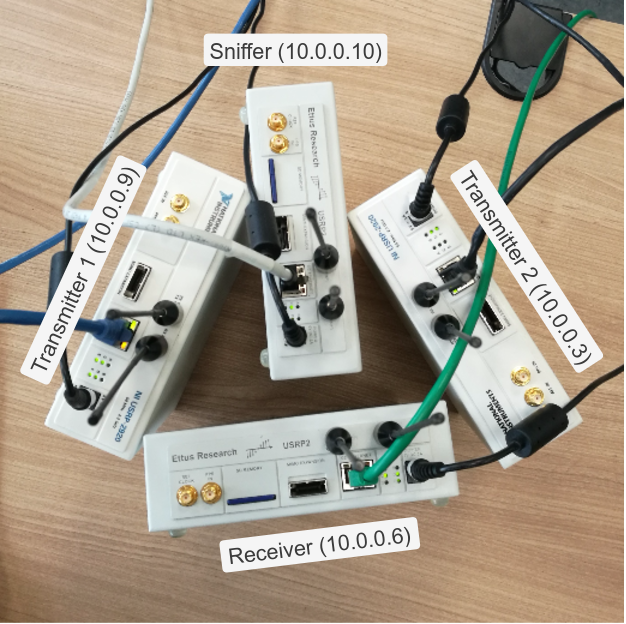
\includegraphics[width=0.5\textwidth]{pictures/measurement_setup}
	\end{center}
	\caption{Photo of the measurement setup.}
\end{figure}

% Measurement parameters
\begin{table}[t]
	\label{tab:measurement-parameters}
	\begin{center}
		\begin{tabular}{p{2.5cm}p{2cm}p{2cm}p{1.5cm}p{1.5cm}p{2cm}}
			\toprule
			Function & TX Gain & RX Gain & Source Address & Dest. Address & IP Address\\
			\midrule
			Receiver 		& 4dB 	& 10dB 	& X 	& any	& 10.0.0.6\\
			Sniffer 		& 0 	& 0 	& any 	& any	& 10.0.0.10 \\
			Transmitter 1 	& 5dB 	& 0 	& Y 	& 	X 	& 10.0.0.9 \\
			Transmitter 2	& 9dB 	& 0 	& Z 	& 	X 	& 10.0.0.3 \\
			\bottomrule	
		\end{tabular}\caption{Setup parameters}
	\end{center}
\end{table}


\section{GNU Radio Flowgraphs}    

\subsection{Receiver and Sniffer}

Figure \ref{fig:grc-receiver} shows the two-way handshake receiving logic. After frame integrity is checked and type is confirmed to be data frame an acknowledgment is generated. The \code{frame\_probe} blocks record the times when the frames reach certain positions in the flowgraph representing the occurrence of events such as frame reception, passed or failed frame integrity check and more. Note that the address check is disabled so that the receiver may receive frames from any sender.

The sniffer consists only of a single \code{frame\_probe} block, which records detected power above noise level during the whole measurement. The sniffer provides valuable insight of what is actually going on in the channel from a "neutral" point of view. Neutral in the sense of:

\begin{itemize}
	\item A clear distinction between the senders can be made according to the energy levels, since the sniffer is located between the senders and transmission gains were chosen accordingly.
	\item Sensing the channel is possible during the whole measurement time, because the sniffer is never sending.
\end{itemize}

In a nutshell, the sniffer is a valuable debugging and verification tool as described in more detail in section \ref{sec:measurement-metrics}.

\begin{sidewaysfigure}[ht]
	\label{fig:grc-receiver}
	\begin{center}
		\subfloat[Receiver]{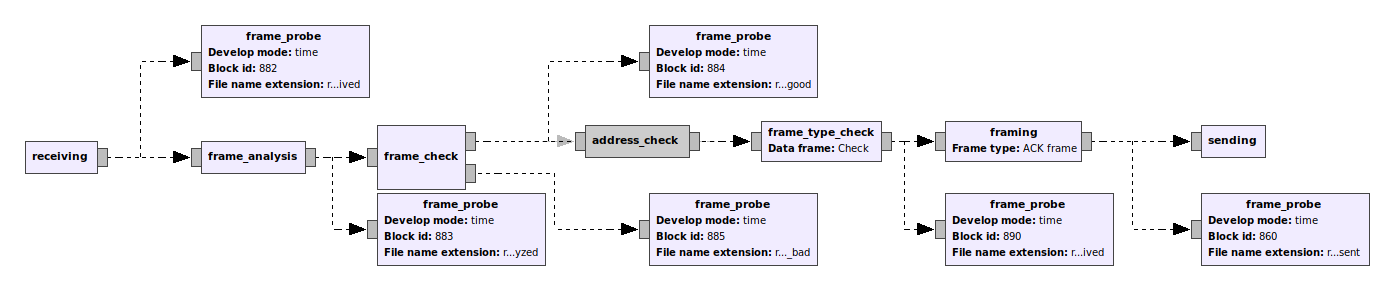
\includegraphics[width=\textwidth]{pictures/grc_receiver_flowgraph}}
		\vskip 40pt
		\subfloat[Sniffer]{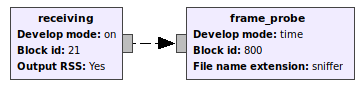
\includegraphics[width=0.3\textwidth]{pictures/grc_sniffer_flowgraph}}
	\end{center}
	\caption{GRC Receiver Flowgraphs}
\end{sidewaysfigure}

\subsection{Pure ALOHA Transmitter}
The \code{run} block enables us to start several senders exactly at the same time, which is useful if we execute the flowgraphs manually without the automated measurement scripts. Payload is generated in the \code{dummy\_source} block, packed into a frame in the \code{framing} block and buffered in the \code{frame\_buffer} block. The interval between generated frames is determined a \code{general\_timer} block, which we trigger either in constant or exponentially distributed intervals. Self-reception is prevented by shutting down the receiver when about to send a frame through the sending block. As soon as the data packet is sent off the \code{timeout} block receives a copy of the data frame. If the timeout timer is reset by a recevied ACK before it runs out the next frame in the buffer is dequeued, otherwise the data is forwarded to the \code{resend\_check} block. If the maximum number of retransmissions, in our case 6 has not been reached a retransmission is issued, otherwise the frame is dropped without substitution.

\begin{sidewaysfigure}[h]
	\label{fig:grc-aloha-sender}
	\begin{center}
		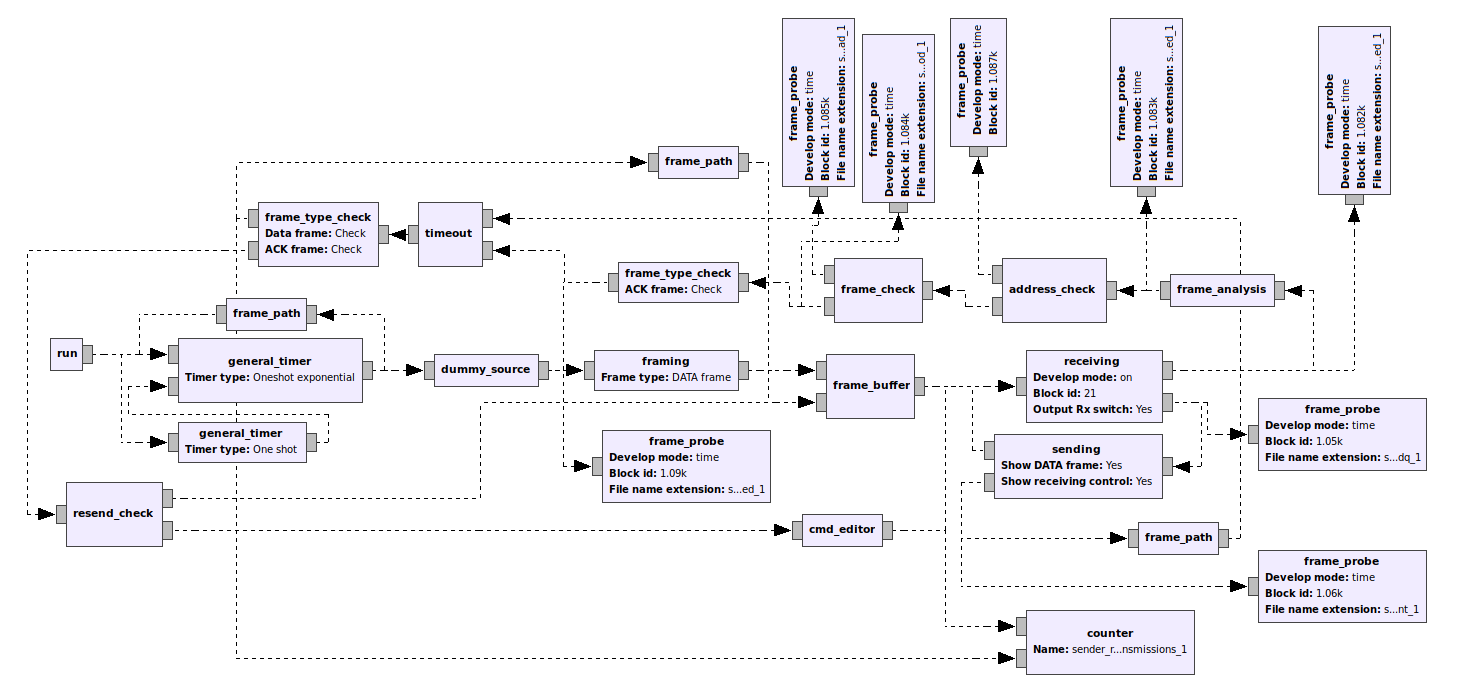
\includegraphics[width=\textwidth]{pictures/grc_aloha_transmitter_flowgraph}
\end{center}
\caption{GRC Pure ALOHA Transmitter Flowgraph}
\end{sidewaysfigure}

\subsection{CSMA Transmitter}

The CSMA transmitter is based on the ALOHA transmitter, but features extra mechanisms as described in section \ref{sec:csma}, which will now be discussed. The flowgraph aims at resembling IEEE 802.11 DCF and features CCA through thresholding in the \code{carrier\_sensing} block. Despite the fact that this block has the feature of adaptively determining an appropriate carrier sensing threshold we chose a fixed value of 0.002 power units (PU) \footnote{Power unit is a linear-scale unit read out via the UHD driver.}. This choice was made to make sure that ALOHA transmission power levels were not confused with noise during the adaptive CSMA noise floor detection period. 

DIFS and SIFS are realized through \code{general\_timer} blocks with the respective values. The design, as depicted, does not feature the RTS/CTS exhange.

\begin{sidewaysfigure}[h]
	\label{fig:grc-csma-sender}
	\begin{center}
		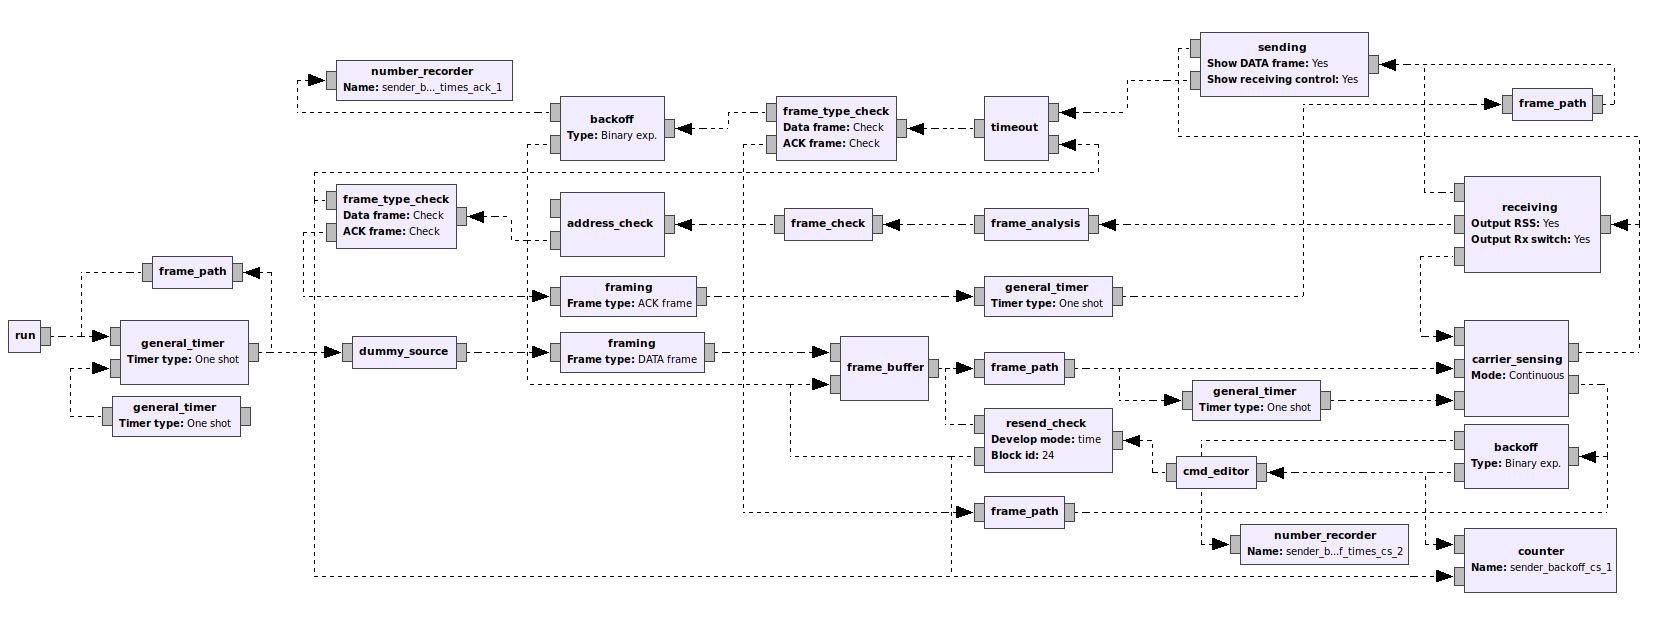
\includegraphics[width=\textwidth]{pictures/grc_csma_transmitter_flowgraph}
\end{center}
\caption{GRC CSMA Transmitter Flowgraph}
\end{sidewaysfigure}

\clearpage

\section{Measurement Metrics}
\label{sec:measurement-metrics}

All recorded metrics will be defined in this section. Furthermore, we will describe the way how they were obtained and how we verified them. All metrics were originally captured with at least one of the following blocks: \code{frame\_probe}, \code{counter}, \code{number\_recorder} and \code{time\_probe} as depicted in figures \ref{fig:grc-receiver}, \ref{fig:grc-aloha-sender} and \ref{fig:grc-csma-sender}.

\subsection{Throughput}

We define throughput as the mean useful data \footnote{payload and headers disregarding retransmissions} transmission rate in the unit kbit/s. We obtain this metric simply by counting the number of ACKs received at the sender, multiply it with the frame length of 8 kbits and divide it by the measurement duration. The calculations are done in \code{throughput.py} making use of the CLI tool \code{wc} to count lines. Joint and single throughputs are our main metrics to judge a protocol's efficiency or how well a certain combination of protocols can coexist under different conditions, respectively.

\subsection{Round-Trip Time}

We define round-trip time (RTT) as the mean time from the buffer dequeuing a data frame until ACK reception. If the variable \code{rtt\_mode} is set to \code{rtt} then this calculation excludes retransmitted frames. If \code{rtt\_mode} is set to \code{frame\_delay} instead then retransmitted frames are taken into account. How we obtain these metrics is best explained with the code in Listing \ref{lst:rtt}, where \code{ack\_received\_times} and \code{data\_sent\_times} contain the timestamps of the frames. 

\begin{lstlisting}[language=Python, caption=The method used in \code{rtt\_alternative.py} to calculate rtt and frame\_delay,label=lst:rtt]
# pointer onto data frame which we use for frame delay calculation
data_pos = 0
for k,ack in enumerate(ack_received_times):
    for l,data in enumerate(data_sent_times):
		# go to 1st data frame that is sent after the respective ack 
        if data > ack:
            if self.rtt_mode == "rtt":
				# the data frame before current position l 
				# must be the frame the ack corresponds to
                rtt_single_measurement += [round(ack - data_sent_times[l-1],5)]
            if self.rtt_mode == "frame_delay":
				# the pointer onto our frame delay reference
				# is used to calculate frame delay
                rtt_single_measurement += [round(ack - data_sent_times[data_pos], 5)]
			# set new reference point for frame delay calculation
            data_pos = l
			# break loop to look at next ack frame!
            break
\end{lstlisting} 

Another way to calculate the RTT is by recording the number of retransmissions of each data frame and subtracting the element with the correct offset in \code{data\_sent\_times} from each ACK reception time. We will not show any code (which can be found in \code{rtt.py}) here, because this has not been used to create any of the plots, although it has been verified to return the same results as the first method. 

\subsection{Packet Loss and Retransmissions per Frame}

Obtaining both metrics involves data processed in \code{rtt.py}, which is why they are calculated there as well. Specifically, we make use of the lists containing the timestamps of ACKs and data frames as well as the number of retransmissions per frame. 
We define packet loss as $ 1 - \frac{n_\text{ACKs}}{n_\text{data}} $, where $ n_\text{ACKs} $ and $ n_\text{data} $ are the number of ACK packets received and data packets sent by the transmitter.
Retransmissions per frame are obtained simply by recording them with a \code{counter} block, which is incremented whenever the \code{timeout} runs out and reset when an ACK is received.

\subsection{Backoff Times}

The script \code{backoff.py} sums up three different backoff times: Firstly, the backoff due to failed \footnote{by failed we mean a negative CCA, i.e. a busy channel.} carrier sensing. Secondly, we capture the backoff times due to successful transmission to give other nodes a chance to seize the channel. Lastly, we sum up the two to obtain the total backoff. The total backoff duration in our view reflects the efficiency of the CSMA protocols in dependency on the parameters DIFS, SIFS and backoff slot length \footnote{E.g. for two CSMA transmitter it would be ideal to have both transmitters back off for around 50\% of the transmission time to give each other a chance to transmit.}. We chose a minimum contention window of $2^5=32$ backoff slots with binary exponential increase. 

\subsection{Packet Durations \& Channel Occupation}

The channel occupation chart as in figure \ref{fig:channel-occupation-example} provides an approximated logical view on the channel in the fashion of a Gantt chart. Blue patches represent data frames, red patches ACKs and black patches the reception of ACKs. The chart is only a (good) approximation of the channel because the width of the patches are fixed and defined in \code{channel\_occupation.py}. The duration of DATA and ACK frames was previously recorded with the \code{time\_probe} blocks as the difference between the times when the frame was dequeued from the buffer and when it was received by the receiver. As expected, the frame durations were very stable. A data frame took 40ms to transmit and an ACK frame took 7ms. The variation of frame length was in the range of 1-2  milliseconds for data frames and in the sub-millisecond range for ACK frames. Depending on the time-limits chosen for the plot this may be well below the plot's resolution, which is why the time axis of such plot will be limited to a range of a few seconds at most.

\subsection{Channel Energy Level}

The energy levels (denoted in a linear-scale, non-negative power unit) in the channel observed by the sniffer (and processed in \code{sniffer.py}) help us to verify a multitude of metrics. We can verify frame durations, round-trip time, backoff time (for saturated traffic) and logical channel occupation. Even collisions are clearly visible and which sender caused them. Throughput ratio among senders can easily be verified by opting in data representation as CDF, e.g. if two identical MAC protocols run under identical circumstances then we expect a CDF with a step where the height of the "energy columns" to the left and right have equal height, i.e. both senders have sent an equal number of data packets.

\subsection{Additional Measures}

\section{Measurement Script System}
\label{sec:script-system}

The elaborate script-system was an integral part of the work and enables future users to much more quickly gain results based on automation, since it is no longer necessary to manually execute flowgraphs, manage captured files, run data processing scripts, sync files with github \ldots Instead everything is automatically done for them. Literally the transmission of every frame and data processing step can be traced back with the log files. Furthermore, to accommodate the need for comparison a retrospective evaluation of any set of measurements \code{belated\_evaluation.py} was created. The user only needs to add a few lines to the script as shown in listing \ref{lst:belated-evaluation-example}.
  
\begin{lstlisting}[language=Python,caption=Evaluation of measurements with \code{belated\_evaluation.py}. In \code{links} we denote the link we used in the corresponding measurement (compare figure \ref{fig:measurement-setup}),label=lst:belated-evaluation-example]
measurement     = [714,715,728,646]
links           = [1,2,1,2]
boxplot_xticks  = [
	"CSMA\nDIFS=15ms\nSIFS=0ms\nBO=0ms\nLink 1 @ 450MHz",
    r"unsaturated ALOHA ~ Poisson($1/\lambda=200ms$), Link 2 @ 450MHz",
    "CSMA\nDIFS=15ms\nSIFS=0ms\nBO=0ms\nLink 1 @ 450MHz\n Baseline",
    "unsaturated ALOHA\nLink 2 @ 450MHz\n Baseline",
]
\end{lstlisting}

\begin{figure}[tb]
	\label{fig:script-system}
	\begin{center}
		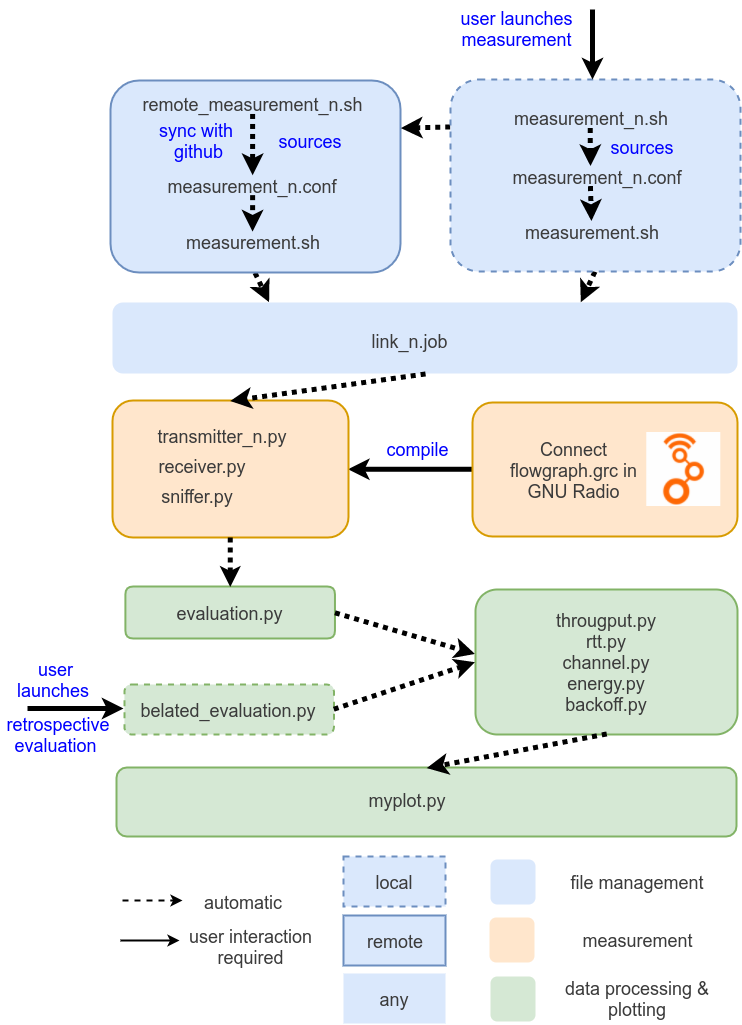
\includegraphics[width=0.8\textwidth]{pictures/script_system}
	\end{center}
	\caption{The three-phase measurement script system. Starting with the user calling \code{measurement\_n.sh}, where n is the ID of the link, general settings are "imported" from \code{measurement\_n.conf}. If the user sets \code{remote\_measurement} to 1 in the conf file then \code{remote\_measurement\_n.sh} synchronizes the files on the remote machine with the github repository, then executes \code{measurement\_n.sh} remotely. Subsequently, \code{measurement.sh} for link n works on open "jobs" from the \code{jobs\_open\_n} directories and optionally puts them into the \code{jobs\_done\_n} directory after completion. In the job files important variables such as duration, repetitions and flowgraph scripts of the measurement are defined. Any variable set in the conf file can be overwritten in the job file since they both are just exporting variables and were separated for semantic reasons only. After the measurement concluded \code{evaluation.py} coordinates data processing which eventually leads to plotting based on Matplotlib as defined in \code{myplot.py}.}
\end{figure}

